% ====================================================================
%  SECCIONES 1–6
% ====================================================================

\section{Antecedentes}
Igualab es una organización peruana dedicada a la consultoría en Diversidad e Inclusión (DEI), sostenibilidad y Responsabilidad Social Empresarial (RSE), enfocada en promover entornos laborales inclusivos y prácticas ASG (Ambiental, Social y Gobernanza) en el sector empresarial peruano. Fundada en 2016, cuenta con certificaciones como Entidad Perceptora de Donaciones (EPD) y reconocimientos internacionales como el Corporate Live Wire Innovation \& Excellence Awards.

En el contexto peruano, las empresas que cotizan en la Bolsa de Valores de Lima (BVL) ---del orden de 115 emisores--- están obligadas a emitir memorias anuales financieras, mientras que los reportes de sostenibilidad son validados por auditores internacionales bajo estándares como el GRI (Global Reporting Initiative). Estos documentos contienen información crítica sobre cumplimiento normativo, sanciones económicas, indicadores de gobernanza y métricas de desempeño ambiental y social.

\textbf{Problemática.} Hoy Igualab opera de manera reactiva en su área comercial: recibe empresas de forma orgánica y no cuenta con herramientas que sistematicen el análisis de la información pública para detectar oportunidades de acercamiento. Buscar, leer y comparar manualmente memorias y reportes (que suelen exceder las 100 páginas) es lento, no es trazable y no escala al universo de emisores de la BVL.

Frente a ello, se plantea el desarrollo de una plataforma web basada en inteligencia artificial (RAG) que permita procesar reportes de sostenibilidad y memorias anuales, identificar brechas en indicadores ASG/GRI y generar información procesada que facilite la toma de decisiones comerciales.

\section{Objetivo General}
Desarrollar una plataforma web de analítica de sostenibilidad que permita a Igualab procesar y consultar información pública de empresas (reportes de sostenibilidad y memorias anuales de la Bolsa de Valores de Lima), identificando brechas en indicadores ASG mediante un asistente de inteligencia artificial (RAG), para impulsar la prospección comercial de la organización de manera proactiva y fundamentada en datos.

\subsection{Objetivos específicos}
\begin{enumerate}[leftmargin=1.6em,itemsep=4pt,topsep=4pt]
  \item Diseñar la arquitectura de la plataforma que integre la información pública de las empresas (memorias anuales y reportes de sostenibilidad) y habilite su explotación mediante inteligencia artificial, asegurando escalabilidad, confiabilidad y eficiencia en el uso de recursos.
  \item Implementar la autenticación y el control de acceso por roles (RBAC) con dos perfiles ---SuperAdmin (gestión) y Administrador (explotación analítica)---, garantizando la seguridad y la trazabilidad de las operaciones.
  \item Desarrollar el módulo de ingesta que permita al SuperAdmin cargar documentos en Markdown (.md) y los deje indexados para su consulta por el Administrador a través de la inteligencia artificial.
  \item Implementar el asistente de inteligencia artificial (RAG) que permita al Administrador consultar en lenguaje natural los documentos ingestados, apoyando la identificación de brechas en códigos GRI y de sanciones económicas, y citando siempre la fuente de la información.
  \item Desarrollar la generación de reportes de prospección en formato PDF a partir de las brechas GRI y sanciones ya validadas, incluyendo un resumen ejecutivo y el puntaje ESG.
  \item Establecer el sistema de auditoría que registre los eventos sensibles (inicios de sesión, cambios de rol, ingesta de datos y generación de reportes) para garantizar la trazabilidad y el cumplimiento de las políticas de seguridad.
\end{enumerate}

\section{Alcance del Proyecto}
El proyecto comprende el diseño, desarrollo e implementación de una plataforma web que centralice la ingesta, indexación, consulta y explotación analítica de memorias anuales y reportes de sostenibilidad (GRI) de empresas que cotizan en la Bolsa de Valores de Lima (BVL), mediante una arquitectura cliente-servidor y un motor de inteligencia artificial basado en RAG (Retrieval-Augmented Generation). Este documento detalla el alcance de la \textbf{FASE 1} (primera versión del software).

\subsection{Roles del sistema}
El sistema está orientado a optimizar las operaciones de dos perfiles (acta CS3081-004-2026 · REQ-10):

\begin{itemize}[leftmargin=1.4em,itemsep=2pt,topsep=2pt]
  \item \textbf{SuperAdmin (1 persona):} gestiona las cuentas de la plataforma (creación, habilitación y deshabilitación, y transferencia del rol) y es responsable del catálogo de empresas y de la ingesta de documentos de sostenibilidad y memorias anuales al sistema.
  \item \textbf{Administrador (2 personas):} realiza consultas al asistente de inteligencia artificial (RAG), revisa y valida las brechas GRI y sanciones, y genera reportes de prospección comercial en formato PDF.
\end{itemize}

El SuperAdmin concentra tanto la administración de accesos como la carga de información fuente, mientras que el Administrador se enfoca exclusivamente en la explotación analítica y comercial de dicha información.

\subsection{Sectores en alcance}
Por acuerdo con el cliente, el análisis de brechas GRI y sanciones se limita a tres sectores: \textbf{Minería, Petróleo y Gas, y Energía} (acta CS3081-003-2026 · REQ-07). Las empresas de otros sectores quedan fuera del análisis y de la generación de reportes en la FASE 1.

\subsection{Fuera de alcance de la FASE 1}
Se declaran explícitamente fuera del alcance de la FASE 1 las siguientes funcionalidades, por decisión del cliente registrada en acta:

\begin{center}
\begin{tabular}{|L{5.4cm}|L{9.6cm}|}
\hline
\thd{Excluido de la FASE 1} & \thd{Referencia (acta)} \\
\hline
Módulo de la Bolsa de Valores (y sus CU/RF asociados) & acta CS3081-005-2026 · REQ-16 \\
\hline
Búsqueda de contactos vía LinkedIn & acta CS3081-005-2026 · REQ-17 \\
\hline
Dashboards de visualización (KPIs ASG/ESG) & acta CS3081-005-2026 · REQ-19 \\
\hline
Portal público y chatbot/asistente vocal & actas CS3081-001 y 002 (FASE 2) \\
\hline
Usuarios ``Cliente'' (multi-tenant) y pasarela de pagos & acta CS3081-004-2026 · REQ-12 \\
\hline
Despliegue a producción (operación en el entorno universitario) & acta CS3081-004-2026 · REQ-11 \\
\hline
\end{tabular}
\end{center}

\subsection{Nota de terminología}
En este documento, \textbf{FASE 1} y \textbf{FASE 2} designan \textbf{versiones del software} (FASE 1 = primera versión, la que aquí se detalla; FASE 2 = versión futura). No deben confundirse con las \textbf{cuatro fases de desarrollo} del Plan de Proyecto v1.2 (Inicial, Análisis y Diseño, Desarrollo, Cierre), que describen la metodología de ejecución del proyecto.

% --------------------------------------------------------------------
\section{Diseño Funcional Detallado}
La solución consiste en una plataforma web de analítica de sostenibilidad que permite a Igualab procesar reportes de sostenibilidad y memorias anuales de empresas que cotizan en la Bolsa de Valores de Lima, identificar brechas en indicadores ASG mediante inteligencia artificial y generar reportes de prospección comercial. La plataforma se estructura como un \textbf{monolito modular} sobre dos roles ---SuperAdmin y Administrador---, organizado en \textbf{ocho módulos funcionales} y un componente transversal de configuración.

\subsection{Criterios de diseño y modularización}
Conforme a los fundamentos de diseño ---modularidad, abstracción, acoplamiento y cohesión--- y a los principios \textbf{SOLID}, el sistema se descompone en módulos de grano fino y responsabilidad única:

\begin{itemize}[leftmargin=1.4em,itemsep=2pt,topsep=2pt]
  \item \textbf{Modularidad:} cada módulo agrupa una responsabilidad funcional y puede evolucionar y probarse de forma independiente.
  \item \textbf{Abstracción:} los servicios exponen interfaces estables y ocultan los detalles de implementación (proveedor de IA, almacenamiento, correo).
  \item \textbf{Alta cohesión y bajo acoplamiento:} cada módulo es dueño único de sus datos y se comunica mediante interfaces bien definidas.
  \item \textbf{Aplicación de SOLID en Igualab:} cada módulo se implementa con un único servicio de responsabilidad única y su propio conjunto de datos; las integraciones externas (proveedor de IA y servicio de correo) se resuelven mediante interfaces sustituibles; cada servicio expone solo las operaciones que su consumidor requiere; y la configuración se inyecta por variables de entorno, no desde implementaciones concretas. En concreto:
    \begin{itemize}[leftmargin=1.2em,itemsep=2pt,topsep=2pt]
      \item \emph{Responsabilidad única:} un servicio por módulo (\texttt{auth\_service}, \texttt{ingesta\_service}, \texttt{gri\_analisis\_service}, \texttt{rag\_chat\_service}, \texttt{reportes\_pdf\_service}, \texttt{auditoria\_service}); la autenticación no se mezcla con la ingesta ni con los reportes.
      \item \emph{Abierto/cerrado:} cambiar de proveedor de IA o de correo no obliga a modificar los servicios, porque se accede a ellos por interfaz.
      \item \emph{Sustitución:} las implementaciones de \texttt{LlmClient} y \texttt{EmbeddingClient} (proveedor \emph{free} y respaldo) son intercambiables sin tocar el código que las consume.
      \item \emph{Segregación de interfaces:} cada módulo publica únicamente las operaciones que su consumidor necesita (por ejemplo, la auditoría es de solo lectura para el SuperAdmin).
      \item \emph{Inversión de dependencias:} los servicios dependen de abstracciones (repositorios y cliente de IA) y la configuración entra por variables de entorno (\texttt{LLM\_*}, \texttt{EMBEDDING\_*}, \texttt{UPLOAD\_MAX\_MB}).
    \end{itemize}
\end{itemize}

\noindent\textbf{Decisión de despliegue:} la FASE 1 se implementa como un monolito modular (una sola unidad desplegable, con los módulos separados internamente); no se adoptan microservicios en esta versión.

\subsection{Catálogo de módulos funcionales}
Cada módulo indica el servicio que lo implementa (SRP), su caso de uso y los requisitos que cubre.

\begin{center}
\begingroup\small
\begin{longtable}{|C{0.7cm}|L{4.4cm}|C{1.4cm}|L{7.8cm}|}
\hline
\thd{\#} & \thd{Módulo / Servicio (SRP)} & \thd{CU} & \thd{Requisitos (RF · RN · RNF)} \\
\hline
\endhead
1 & Autenticación y Gestión de Sesión --- \texttt{auth\_service} & CU001 & RN-001…RN-013 · RF-001…RF-005 · RNF-001…RNF-009 \\
\hline
2 & Gestión de Usuarios --- \texttt{usuario\_service} & CU002 & RN-001…RN-009 · RF-006…RF-009 · RNF-012, RNF-013 \\
\hline
3 & Catálogo de Empresas --- \texttt{empresa\_service} & CU003 & RN-014…RN-017 · RF-010, RF-011 · --- \\
\hline
4 & Ingesta de Documentos --- \texttt{ingesta\_service} & CU003 & RN-018…RN-026 · RF-012…RF-017 · RNF-007, RNF-011, RNF-015, RNF-016, RNF-020, RNF-025, RNF-029, RNF-031 \\
\hline
5 & Análisis y Validación de Brechas GRI --- \texttt{gri\_analisis\_service} & CU005 & RN-027…RN-032 · RF-018…RF-022, RF-027 · RNF-014, RNF-026, RNF-027 \\
\hline
6 & Asistente de IA (RAG) --- \texttt{rag\_chat\_service} & CU004 & RN-033…RN-037 · RF-023, RF-024 · RNF-010, RNF-017, RNF-018, RNF-019 \\
\hline
7 & Generación de Reportes de Prospección --- \texttt{reportes\_pdf\_service} & CU006 & RN-038…RN-041 · RF-025, RF-026 · --- \\
\hline
8 & Auditoría Funcional --- \texttt{auditoria\_service} & CU007 & RN-042…RN-045 · RF-028 · RNF-022, RNF-023, RNF-024 \\
\hline
--- & Configuración (transversal, sin módulo propio) & --- & Parámetros por variables de entorno: tamaño máximo de ingesta y cuota del proveedor de IA (RNF-020, RNF-027) \\
\hline
\end{longtable}
\endgroup
\end{center}

\noindent{\small La numeración de CU y de requisitos corresponde a la del presente documento (secciones 6 y 7).}

\subsection{Descripción de los módulos}

\subsubsection{Módulo 1 --- Autenticación y Gestión de Sesión}
Controla el acceso a la plataforma mediante correo y contraseña, garantizando que solo cuentas registradas y habilitadas puedan operar el sistema. Contempla la recuperación de contraseña por enlace temporal de un solo uso, el cambio de contraseña estando autenticado, la expiración de sesión por inactividad, el cierre de sesión manual y el bloqueo temporal de la cuenta tras 5 intentos fallidos consecutivos. La sesión se soporta con un token JWT firmado que incorpora la identidad de la cuenta, mientras que el rol vigente se valida en cada petición.

\subsubsection{Módulo 2 --- Gestión de Usuarios}
Exclusivo del SuperAdmin: permite crear cuentas de Administrador (con contraseña temporal para el primer acceso), habilitarlas o deshabilitarlas ---invalidando de inmediato sus sesiones activas--- y transferir el rol SuperAdmin a una cuenta de Administrador existente y habilitada, con confirmación previa y ejecución atómica. El sistema garantiza en todo momento la existencia de exactamente una cuenta con rol SuperAdmin y no contempla eliminación permanente de cuentas, solo habilitación y deshabilitación, para preservar la trazabilidad de auditoría.

\subsubsection{Módulo 3 --- Catálogo de Empresas}
Exclusivo del SuperAdmin: registra las empresas sobre las cuales se realizará el análisis, exigiendo nombre y sector. El sector es un atributo de la empresa y pertenece a un conjunto cerrado de tres valores (Minería, Petróleo y Gas, y Energía); las empresas de otros sectores no son elegibles para el análisis ni para la generación de reportes.

\subsubsection{Módulo 4 --- Ingesta de Documentos}
Exclusivo del SuperAdmin: carga memorias anuales y reportes de sostenibilidad GRI en formato Markdown (.md), asociados obligatoriamente a una empresa, un año y un tipo de documento. El sistema valida el tipo real del archivo en el servidor, calcula su hash SHA-256 para rechazar duplicados y verifica que contenga al menos un código GRI o una mención de sanción reconocible; en caso contrario, el documento se marca como observado en lugar de rechazarse por completo. El procesamiento es síncrono, con progreso visible al usuario, e incluye la indexación del contenido y la ejecución automática del análisis de brechas GRI como último paso de una ingesta exitosa. Ante rechazo o interrupción, el sistema revierte el procesamiento sin conservar contenido parcial.

\subsubsection{Módulo 5 --- Análisis y Validación de Brechas GRI}
Exclusivo del Administrador: traduce el contenido indexado en un diagnóstico de cumplimiento GRI con supervisión humana obligatoria. El motor identifica automáticamente qué códigos del catálogo GRI (40 códigos) están presentes en el documento, citando el fragmento de origen, sin comparar contra el texto del estándar GRI oficial. El Administrador revisa cada cita textual y asigna manualmente el estado del código (OK, Baja sustancia o Sub-reportado); el sistema no infiere ni calcula este estado de forma automática. Las sanciones económicas se identifican exclusivamente a partir de menciones explícitas en los documentos ingestados. El puntaje ESG se calcula a partir de los estados asignados; si no se detectó ningún código, se muestra como ``no disponible'', nunca como cero.

\subsubsection{Módulo 6 --- Asistente de Inteligencia Artificial (RAG)}
Exclusivo del Administrador: permite consultas en lenguaje natural sobre el corpus indexado, requiriendo seleccionar sector, empresa y año antes de habilitar la consulta. El asistente se limita a responder sobre sostenibilidad empresarial, indicadores GRI, sanciones o el contenido de los documentos ingestados; ante cualquier otra consulta declina explícitamente. Toda respuesta incluye la referencia al documento, empresa y año de origen, y suprime cualquier afirmación sin fuente verificable en el corpus; ante información insuficiente, lo declara en lugar de inventar una respuesta. El contenido recuperado se trata siempre como datos de referencia dentro del prompt, nunca como instrucciones del sistema. Ante indisponibilidad del proveedor externo de IA, informa el error sin bloquear el resto de los módulos.

\subsubsection{Módulo 7 --- Generación de Reportes de Prospección}
Exclusivo del Administrador: consolida el análisis validado de una empresa en un documento PDF para el acercamiento comercial. Solo puede generarse para empresas con al menos un documento indexado y se construye exclusivamente a partir de los resultados de análisis ya almacenados y validados manualmente, sin invocar al servicio de IA en este paso, por lo que dos generaciones sobre los mismos datos producen el mismo resultado. El reporte incluye el estado de cada código GRI con su cita de respaldo, las sanciones identificadas (con monto o marcadas como ``no cuantificada'') y un resumen ejecutivo con el puntaje ESG. Una vez generado, el reporte es inmutable; su historial es visualizable y descargable por cualquier Administrador.

\subsubsection{Módulo 8 --- Auditoría Funcional}
Exclusivo del SuperAdmin: registra automáticamente todo evento sensible del sistema ---inicio de sesión, cambio de estado o rol de cuenta, ingesta, rechazo de documento y generación de reportes---, consignando la cuenta responsable, la fecha y hora (UTC) y el tipo de acción. El registro es consultable filtrando por usuario, fecha y tipo de evento, y es de solo inserción: no admite edición ni eliminación.

\subsection{Flujos funcionales end-to-end}
\begin{itemize}[leftmargin=1.4em,itemsep=3pt,topsep=2pt]
  \item \textbf{F1 · Ingesta y análisis (SuperAdmin):} autenticarse $\rightarrow$ seleccionar sector y empresa, año y tipo $\rightarrow$ subir el \texttt{.md} $\rightarrow$ \emph{guard} (extensión, tamaño, hash) $\rightarrow$ parseo y chunking $\rightarrow$ \emph{embeddings} por API $\rightarrow$ indexación $\rightarrow$ detección de códigos GRI y sanciones (filas sin estado) $\rightarrow$ auditoría $\rightarrow$ resultado con progreso.
  \item \textbf{F2 · Consulta RAG (Administrador):} seleccionar sector, empresa y año $\rightarrow$ formular la pregunta $\rightarrow$ recuperación semántica $\rightarrow$ respuesta del modelo con citas (o declinación fuera de dominio).
  \item \textbf{F3 · Revisión de brechas (Administrador):} abrir las filas con su cita $\rightarrow$ asignar el estado manual $\rightarrow$ registrar el histórico.
  \item \textbf{F4 · Reporte de prospección (Administrador):} verificar estados validados $\rightarrow$ generar el PDF determinista (sin IA) $\rightarrow$ snapshot inmutable $\rightarrow$ auditoría $\rightarrow$ historial y descarga.
  \item \textbf{F5 · Autenticación y usuarios (SuperAdmin):} iniciar sesión o recuperar contraseña; crear, habilitar/deshabilitar y transferir el rol SuperAdmin (atómico).
  \item \textbf{F6 · Auditoría (SuperAdmin):} consultar y filtrar los eventos; solo lectura.
\end{itemize}

\subsection{Reglas transversales de diseño}
\begin{enumerate}[leftmargin=1.6em,itemsep=2pt,topsep=2pt]
  \item \textbf{RBAC de dos roles} en cada endpoint (autorización por petición; el rol se valida en el servidor).
  \item \textbf{Ingesta síncrona} de \texttt{.md} (tablas con pipes), con hash y \textbf{reversión atómica} ante fallo.
  \item \textbf{Tres estados GRI}, asignación 100\,\% manual; el puntaje ESG se deriva y es ``no disponible'' si no hay códigos.
  \item \textbf{RAG simple} sin \emph{function calling}; citación obligatoria; el corpus se trata como datos (anti \emph{prompt injection}); \emph{timeout} de IA de 1 minuto.
  \item \textbf{Reporte determinista sin IA} e inmutable.
  \item \textbf{Auditoría append-only} en UTC.
  \item \textbf{Trazabilidad:} cada módulo referencia sus CU $\leftrightarrow$ RF $\leftrightarrow$ RN $\leftrightarrow$ RNF (tabla anterior).
\end{enumerate}

% --------------------------------------------------------------------
\section{Diagrama del Proceso}
En este apartado se presentan los diagramas del proceso: la integración entre los sistemas de la empresa en la situación actual (5.1) y la interoperación con los sistemas externos vinculados con ella en la situación propuesta (5.2).

\subsection{Integración entre los sistemas de la empresa}
En la situación actual (AS-IS), Igualab no integra sistemas para el análisis comercial: el analista realiza todo el proceso de forma manual y reactiva. Busca y descarga cada informe (memoria anual y/o reporte de sostenibilidad) de fuentes dispersas, lo lee íntegramente, identifica brechas, sanciones y oportunidades de mejora, y elabora el documento de prospección en texto libre. No existe una base de datos ni una aplicación que articule estas actividades, por lo que no hay trazabilidad, comparación entre empresas ni reutilización de resultados. La figura siguiente representa el flujo end-to-end actual.

\begin{center}
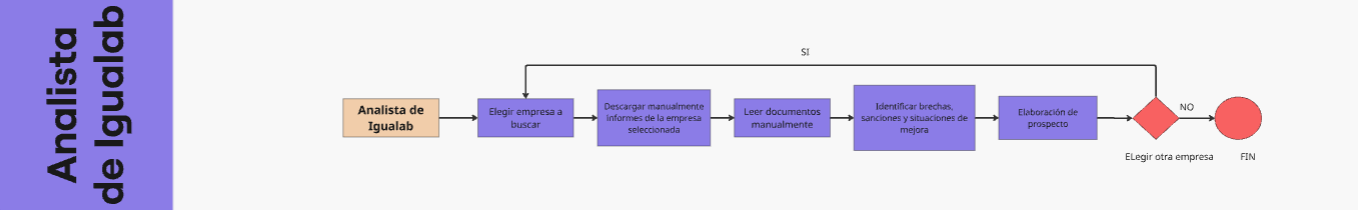
\includegraphics[width=0.94\textwidth]{img/im-011-009.png}
\end{center}

\subsection{Interoperación con sistemas externos vinculados con la empresa}
En la situación propuesta (TO-BE), la plataforma articula internamente el proceso y se comunica con sistemas externos mediante interfaces estandarizadas: el \textbf{proveedor de IA} (embeddings y generación por HTTPS/JSON), el \textbf{servicio de correo} (SMTP, para la recuperación de contraseña) y la \textbf{Bolsa de Valores de Lima (BVL)}, que es la fuente de los documentos y que el cliente entrega ya convertidos a Markdown, sin integración por API. El asistente de IA consume al proveedor externo como un servicio, sin que el modelo decida acciones sobre el sistema, y el contenido recuperado del corpus se trata como datos, nunca como instrucciones. Con ello, el proceso se organiza en los carriles del Sistema (automático), el SuperAdmin (gestión e ingesta) y el Administrador (explotación analítica), e incorpora el análisis GRI y de sanciones y la generación del reporte. La figura siguiente representa el proceso objetivo.

\begin{center}
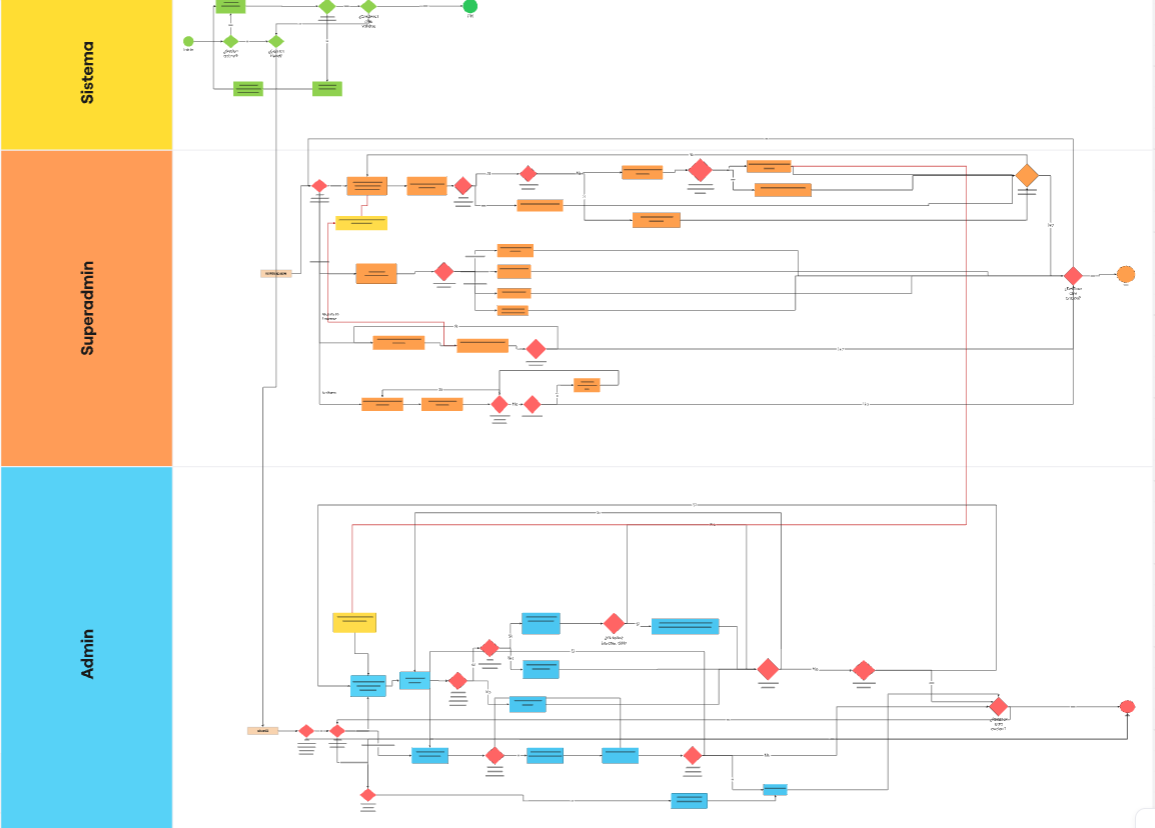
\includegraphics[width=0.96\textwidth]{img/im-012-010.png}
\end{center}
\noindent Enlace del tablero del proceso: \href{https://miro.com/app/board/uXjVHq4p518=/}{https://miro.com/app/board/uXjVHq4p518=/}

% --------------------------------------------------------------------
\section{Reglas de Negocio}
Las Reglas de Negocio (RN) se detallan a continuación, agrupadas por dominio: acceso y cuentas, empresas y sectores, ingesta documental, análisis GRI, asistente IA, reportes de prospección y auditoría.

\begingroup\small
\begin{longtable}{|C{1.4cm}|L{4.0cm}|L{9.4cm}|}
\hline
\thd{RN} & \thd{NOMBRE DE LA REGLA} & \thd{DETALLE DE LA REGLA} \\
\hline
RN-001 & Conjunto cerrado de roles & \textbf{SI} una cuenta opera en la plataforma, \textbf{ENTONCES} el sistema le reconoce exactamente uno de dos roles ---SuperAdmin o Administrador--- y aplica únicamente los permisos de ese rol. \textbf{SE APLICA A} todas las cuentas y a todos los módulos y endpoints de la plataforma. \textbf{SE BASA EN} el modelo RBAC de dos roles acordado con el cliente (acta CS3081-004-2026 · REQ-10) y en el principio de mínimo privilegio. \textbf{Y TIENE LA SIGUIENTE EXCEPCIÓN} no se admiten roles adicionales (p. ej. «Usuario») ni cuentas sin rol asignado. \\
\hline
RN-002 & Unicidad del SuperAdmin & \textbf{SI} se crea, habilita, deshabilita o transfiere una cuenta, \textbf{ENTONCES} el sistema garantiza que exista exactamente una cuenta con rol SuperAdmin en todo momento, con independencia de su estado de habilitación o de si mantiene una sesión abierta. \textbf{SE APLICA A} la creación de cuentas, la habilitación/deshabilitación y la transferencia de rol. \textbf{SE BASA EN} el principio de responsabilidad única sobre la administración del sistema y en el acuerdo del cliente (acta CS3081-004-2026 · REQ-10). \textbf{Y TIENE LA SIGUIENTE EXCEPCIÓN} la cuenta SuperAdmin inicial se crea durante el despliegue y no puede crearse desde la aplicación (RN-006). \\
\hline
RN-003 & Permisos cerrados por rol & \textbf{SI} una cuenta intenta ejecutar una acción, \textbf{ENTONCES} el sistema la autoriza únicamente si esa acción corresponde a su rol; en caso contrario, deniega el acceso con error de autorización. \textbf{SE APLICA A} todos los módulos y endpoints, evaluándose en cada petición. \textbf{SE BASA EN} el principio de mínimo privilegio (RBAC). \textbf{Y TIENE LA SIGUIENTE EXCEPCIÓN} no existe excepción por interfaz: ocultar una opción en la pantalla no otorga ni niega permiso, pues la autorización se resuelve en el servidor. \\
\hline
RN-004 & Condiciones de autenticación & \textbf{SI} una cuenta intenta iniciar sesión, \textbf{ENTONCES} el sistema le permite el acceso únicamente si está registrada, se encuentra habilitada y su contraseña es correcta. \textbf{SE APLICA A} todas las cuentas, incluida la cuenta SuperAdmin creada en el despliegue. \textbf{SE BASA EN} el control de acceso por credenciales. \textbf{Y TIENE LA SIGUIENTE EXCEPCIÓN} una cuenta deshabilitada no puede autenticarse aunque sus credenciales sean correctas (RN-005). \\
\hline
RN-005 & Efecto de la deshabilitación de cuenta & \textbf{SI} el SuperAdmin deshabilita una cuenta, \textbf{ENTONCES} el sistema invalida de inmediato todas sus sesiones activas y le revoca el acceso a todas las funcionalidades, sin eliminar su información ni su historial. \textbf{SE APLICA A} las cuentas de Administrador. \textbf{SE BASA EN} la revocación inmediata de accesos y en la conservación de la trazabilidad. \textbf{Y TIENE LA SIGUIENTE EXCEPCIÓN} la cuenta SuperAdmin no puede deshabilitarse desde la aplicación; primero debe transferirse el rol (RN-009). \\
\hline
RN-006 & Cuenta SuperAdmin inicial & \textbf{SI} el sistema se despliega por primera vez, \textbf{ENTONCES} se crea una única cuenta con rol SuperAdmin durante el despliegue, con independencia de la aplicación. \textbf{SE APLICA A} el aprovisionamiento inicial del sistema. \textbf{SE BASA EN} la necesidad de un administrador raíz que no dependa de la interfaz. \textbf{Y TIENE LA SIGUIENTE EXCEPCIÓN} esta cuenta no puede crearse ni eliminarse desde la aplicación; su rol solo se transfiere (RN-009). \\
\hline
RN-007 & Datos obligatorios de la cuenta & \textbf{SI} se registra o edita una cuenta, \textbf{ENTONCES} el sistema exige nombre completo, correo electrónico y contraseña, y valida el formato del correo. \textbf{SE APLICA A} la creación y la edición de cuentas. \textbf{SE BASA EN} la integridad de la identidad de la cuenta. \textbf{Y TIENE LA SIGUIENTE EXCEPCIÓN} no se admite una cuenta sin los tres datos obligatorios ni con un correo ya registrado (unicidad de correo). \\
\hline
RN-008 & Rol por defecto & \textbf{SI} el SuperAdmin crea una cuenta desde la aplicación, \textbf{ENTONCES} el sistema le asigna automáticamente el rol Administrador. \textbf{SE APLICA A} la creación de cuentas. \textbf{SE BASA EN} que el rol SuperAdmin solo se obtiene por transferencia (RN-009). \textbf{Y TIENE LA SIGUIENTE EXCEPCIÓN} no es posible crear cuentas con rol SuperAdmin desde la interfaz. \\
\hline
RN-009 & Transferencia atómica del rol SuperAdmin & \textbf{SI} el SuperAdmin transfiere su rol a una cuenta de Administrador existente y habilitada, \textbf{ENTONCES} el sistema ejecuta la operación de forma atómica, previa confirmación: la cuenta destino adquiere el rol SuperAdmin y la cuenta origen pasa a Administrador en una sola transacción. \textbf{SE APLICA A} la transferencia de rol. \textbf{SE BASA EN} la unicidad del SuperAdmin (RN-002) y en la integridad transaccional. \textbf{Y TIENE LA SIGUIENTE EXCEPCIÓN} si la cuenta destino no existe, está deshabilitada o ya es SuperAdmin, la transferencia se rechaza sin alterar el estado de las cuentas. \\
\hline
RN-010 & Autonomía en la recuperación de acceso & \textbf{SI} un usuario pierde sus credenciales, \textbf{ENTONCES} el sistema le permite recuperar el acceso por sí mismo mediante un enlace seguro enviado a su correo, sin intervención del SuperAdmin. \textbf{SE APLICA A} todas las cuentas habilitadas. \textbf{SE BASA EN} la autonomía del usuario y en la autenticación segura por correo. \textbf{Y TIENE LA SIGUIENTE EXCEPCIÓN} el enlace es de un solo uso y de vigencia limitada (30 minutos); vencido o ya usado, debe generarse uno nuevo. \\
\hline
RN-011 & Política de contraseñas & \textbf{SI} se crea o cambia una contraseña, \textbf{ENTONCES} el sistema exige un mínimo de 8 caracteres con al menos una mayúscula, una minúscula, un dígito y un carácter especial, y no admite que coincida con el correo de la cuenta. \textbf{SE APLICA A} el registro, el cambio y el restablecimiento de contraseña. \textbf{SE BASA EN} las buenas prácticas de autenticación segura. \textbf{Y TIENE LA SIGUIENTE EXCEPCIÓN} no se permite guardar la contraseña en texto plano; su almacenamiento es un hash con sal (RNF). \\
\hline
RN-012 & Bloqueo por intentos fallidos & \textbf{SI} una cuenta acumula 5 intentos fallidos consecutivos de inicio de sesión, \textbf{ENTONCES} el sistema la bloquea temporalmente durante 15 minutos, impide nuevos intentos y registra el evento en la auditoría. \textbf{SE APLICA A} todas las cuentas que se autentican con credenciales. \textbf{SE BASA EN} la mitigación de ataques de fuerza bruta. \textbf{Y TIENE LA SIGUIENTE EXCEPCIÓN} el bloqueo se levanta automáticamente al vencer el tiempo o al restablecerse la contraseña; no requiere intervención manual. \\
\hline
RN-013 & Sesión e inactividad & \textbf{SI} una sesión permanece sin actividad durante 2 horas, \textbf{ENTONCES} el sistema la expira y exige una nueva autenticación; asimismo, el usuario puede cerrar la sesión manualmente. \textbf{SE APLICA A} todas las sesiones autenticadas. \textbf{SE BASA EN} el control de sesiones y en la revocación por inactividad. \textbf{Y TIENE LA SIGUIENTE EXCEPCIÓN} tras una transferencia de rol, la sesión activa aplica el rol vigente; si la cuenta se deshabilita, la sesión se invalida de inmediato (RN-005). \\
\hline
RN-014 & Registro de empresas & \textbf{SI} el SuperAdmin registra una empresa, \textbf{ENTONCES} el sistema exige un nombre y la asignación a un sector. \textbf{SE APLICA A} la creación y edición del catálogo de empresas. \textbf{SE BASA EN} el acuerdo con el cliente (acta CS3081-004-2026 · REQ-10) y en la necesidad de identificar la empresa por su nombre y su sector. \textbf{Y TIENE LA SIGUIENTE EXCEPCIÓN} no se admite una empresa sin nombre ni sin sector. \\
\hline
RN-015 & Sectores habilitados (conjunto cerrado) & \textbf{SI} se registra una empresa o se realiza una ingesta o consulta, \textbf{ENTONCES} el sistema solo admite tres sectores: Minería, Petróleo y Gas, y Energía. \textbf{SE APLICA A} el catálogo de empresas, la ingesta y las consultas. \textbf{SE BASA EN} el acuerdo con el cliente (acta CS3081-003-2026 · REQ-07). \textbf{Y TIENE LA SIGUIENTE EXCEPCIÓN} no se crean sectores nuevos; las empresas de otros sectores pueden registrarse, pero no son elegibles para el análisis ni para la generación de reportes. \\
\hline
RN-016 & Unicidad de la empresa & \textbf{SI} se registra una empresa, \textbf{ENTONCES} el sistema rechaza el registro si ya existe otra con el mismo nombre. \textbf{SE APLICA A} la creación y edición del catálogo de empresas. \textbf{SE BASA EN} la integridad del catálogo. \textbf{Y TIENE LA SIGUIENTE EXCEPCIÓN} no se admiten empresas duplicadas. \\
\hline
RN-017 & Vigencia de la empresa (activa/inactiva) & \textbf{SI} una empresa se marca como inactiva, \textbf{ENTONCES} el sistema deja de ofrecerla para la ingesta y las consultas y no la considera en el análisis. \textbf{SE APLICA A} el catálogo de empresas. \textbf{SE BASA EN} la vigencia del catálogo. \textbf{Y TIENE LA SIGUIENTE EXCEPCIÓN} la empresa inactiva conserva sus documentos y su historial y no se elimina. \\
\hline
RN-018 & Formato de ingesta & \textbf{SI} el SuperAdmin carga un documento, \textbf{ENTONCES} el sistema solo admite archivos Markdown (.md) con tablas de pipes. \textbf{SE APLICA A} la ingesta de memorias anuales y reportes de sostenibilidad. \textbf{SE BASA EN} el acuerdo del cliente (acta CS3081-005-2026 · REQ-20). \textbf{Y TIENE LA SIGUIENTE EXCEPCIÓN} el sistema no convierte formatos distintos de Markdown. \\
\hline
RN-019 & Responsabilidad de la conversión & \textbf{SI} el cliente entrega un documento, \textbf{ENTONCES} es responsable de su conversión a Markdown y de la integridad de sus tablas (formato pipe). \textbf{SE APLICA A} la preparación de los documentos fuente. \textbf{SE BASA EN} la delimitación de responsabilidades acordada. \textbf{Y TIENE LA SIGUIENTE EXCEPCIÓN} el sistema no reconvierte ni corrige el contenido entregado. \\
\hline
RN-020 & Tipos de documento admisibles & \textbf{SI} se carga un documento, \textbf{ENTONCES} su tipo debe ser memoria anual o reporte de sostenibilidad GRI. \textbf{SE APLICA A} la ingesta. \textbf{SE BASA EN} la distinción de los dos documentos fuente del proceso. \textbf{Y TIENE LA SIGUIENTE EXCEPCIÓN} no se admiten otros tipos de documento. \\
\hline
RN-021 & Tamaño máximo de ingesta & \textbf{SI} se carga un documento, \textbf{ENTONCES} el sistema rechaza la carga si el archivo supera los 50 MB. \textbf{SE APLICA A} la ingesta. \textbf{SE BASA EN} el límite acordado para el procesamiento. \textbf{Y TIENE LA SIGUIENTE EXCEPCIÓN} el rechazo se registra con su motivo y no se procesa contenido parcial. \\
\hline
RN-022 & Identificación obligatoria del documento & \textbf{SI} se carga un documento, \textbf{ENTONCES} debe estar asociado a una empresa activa, al año del ejercicio y a su tipo. \textbf{SE APLICA A} la ingesta. \textbf{SE BASA EN} la trazabilidad del documento de origen. \textbf{Y TIENE LA SIGUIENTE EXCEPCIÓN} no se indexa un documento sin empresa, año y tipo. \\
\hline
RN-023 & Unicidad de documento por empresa, año y tipo & \textbf{SI} se carga un documento, \textbf{ENTONCES} el sistema rechaza la carga si ya existe otro del mismo tipo para la misma empresa y año. \textbf{SE APLICA A} la ingesta. \textbf{SE BASA EN} la evitación de duplicados documentales. \textbf{Y TIENE LA SIGUIENTE EXCEPCIÓN} el rechazo indica la fecha y la cuenta que realizó la carga original. \\
\hline
RN-024 & Unicidad por contenido (SHA-256) & \textbf{SI} se carga un documento, \textbf{ENTONCES} el sistema calcula su hash SHA-256 y rechaza la carga si ese contenido ya fue ingestado. \textbf{SE APLICA A} la ingesta. \textbf{SE BASA EN} la detección de duplicados por contenido. \textbf{Y TIENE LA SIGUIENTE EXCEPCIÓN} un documento rechazado o interrumpido no deja contenido en el corpus. \\
\hline
RN-025 & Contenido mínimo y estado observado & \textbf{SI} un documento no contiene al menos un código del catálogo GRI ni una mención de sanción reconocible, \textbf{ENTONCES} el sistema lo marca como observado y no lo indexa hasta corregirse. \textbf{SE APLICA A} la ingesta. \textbf{SE BASA EN} la necesidad de que el documento aporte información analizable. \textbf{Y TIENE LA SIGUIENTE EXCEPCIÓN} el documento observado no se rechaza por completo; se conserva para su reintento. \\
\hline
RN-026 & Integridad atómica de la ingesta & \textbf{SI} una ingesta es rechazada o interrumpida, \textbf{ENTONCES} el sistema revierte el procesamiento y elimina cualquier contenido, fragmento, embedding o resultado generado parcialmente, conservando únicamente el motivo del rechazo. \textbf{SE APLICA A} la ingesta. \textbf{SE BASA EN} la integridad del corpus. \textbf{Y TIENE LA SIGUIENTE EXCEPCIÓN} solo se conserva la información necesaria para identificar y auditar el rechazo. \\
\hline
RN-027 & Catálogo de códigos GRI evaluables & \textbf{SI} el sistema analiza un documento, \textbf{ENTONCES} solo considera los 40 códigos del catálogo GRI corporativo versionado. \textbf{SE APLICA A} el análisis de brechas. \textbf{SE BASA EN} el catálogo acordado con el PO. \textbf{Y TIENE LA SIGUIENTE EXCEPCIÓN} el texto del estándar GRI oficial no es fuente de evaluación; la evidencia válida es la reportada por la empresa. \\
\hline
RN-028 & Detección de códigos y extracción de cita & \textbf{SI} el sistema analiza un documento indexado, \textbf{ENTONCES} identifica los códigos del catálogo presentes y extrae la cita textual de respaldo, sin evaluar su contenido. \textbf{SE APLICA A} el análisis posterior a la ingesta. \textbf{SE BASA EN} la supervisión humana del estado. \textbf{Y TIENE LA SIGUIENTE EXCEPCIÓN} el sistema no compara el contenido contra el texto del estándar GRI. \\
\hline
RN-029 & Asignación manual del estado GRI & \textbf{SI} se detecta un código GRI en el documento, \textbf{ENTONCES} el estado del código es asignado manualmente por el Administrador tras revisar la cita textual. \textbf{SE APLICA A} el análisis y la validación de brechas. \textbf{SE BASA EN} la supervisión humana acordada con el PO. \textbf{Y TIENE LA SIGUIENTE EXCEPCIÓN} el sistema no infiere ni sugiere el estado de forma automática. \\
\hline
RN-030 & Conjunto cerrado de estados GRI & \textbf{SI} el Administrador asigna un estado, \textbf{ENTONCES} solo puede ser uno de tres valores: OK, Baja sustancia o Sub-reportado. \textbf{SE APLICA A} el análisis y la validación de brechas. \textbf{SE BASA EN} los estados acordados con el PO. \textbf{Y TIENE LA SIGUIENTE EXCEPCIÓN} no existe un cuarto estado (p. ej. «Crítico»). \\
\hline
RN-031 & Origen de las sanciones & \textbf{SI} el sistema identifica sanciones, \textbf{ENTONCES} solo las toma de menciones explícitas en los documentos ingestados de la empresa. \textbf{SE APLICA A} el análisis de sanciones. \textbf{SE BASA EN} que el sistema no consulta fuentes externas. \textbf{Y TIENE LA SIGUIENTE EXCEPCIÓN} si la sanción no tiene monto, se conserva como «no cuantificada» y nunca se asume cero (RN-032). \\
\hline
RN-032 & Cálculo del puntaje ESG & \textbf{SI} se asignan estados a los códigos GRI de una empresa y un año, \textbf{ENTONCES} el sistema calcula el puntaje ESG con la fórmula OK = 100, Baja sustancia = 50 y Sub-reportado = 0. \textbf{SE APLICA A} el reporte de prospección. \textbf{SE BASA EN} los estados validados. \textbf{Y TIENE LA SIGUIENTE EXCEPCIÓN} si no se detectó ningún código, el puntaje se muestra como «no disponible», nunca como cero. \\
\hline
RN-033 & Fundamentación en el corpus & \textbf{SI} el Administrador consulta al asistente, \textbf{ENTONCES} el sistema genera la respuesta exclusivamente con base en los documentos ingestados. \textbf{SE APLICA A} las consultas en lenguaje natural. \textbf{SE BASA EN} el acuerdo con el PO (IA delimitada a la base del cliente). \textbf{Y TIENE LA SIGUIENTE EXCEPCIÓN} no se emplea conocimiento externo al corpus. \\
\hline
RN-034 & Trazabilidad de la información entregada & \textbf{SI} el asistente entrega información, \textbf{ENTONCES} toda afirmación debe ser atribuible a un documento del corpus, citando documento, empresa y año. \textbf{SE APLICA A} las respuestas del asistente. \textbf{SE BASA EN} la verificabilidad de la información. \textbf{Y TIENE LA SIGUIENTE EXCEPCIÓN} una afirmación sin respaldo trazable no es información válida del sistema. \\
\hline
RN-035 & Declaración explícita ante ausencia de información & \textbf{SI} el corpus no contiene información suficiente, \textbf{ENTONCES} el asistente lo declara explícitamente en lugar de inventar una respuesta. \textbf{SE APLICA A} las respuestas del asistente. \textbf{SE BASA EN} la honestidad de la respuesta. \textbf{Y TIENE LA SIGUIENTE EXCEPCIÓN} la ausencia de respaldo nunca se sustituye por datos generados o atribuidos a fuentes inexistentes. \\
\hline
RN-036 & Restricción de dominio del asistente & \textbf{SI} la consulta se refiere a un tema fuera de sostenibilidad empresarial, indicadores GRI, sanciones o el contenido ingestado, \textbf{ENTONCES} el asistente declina explícitamente. \textbf{SE APLICA A} todas las consultas. \textbf{SE BASA EN} el alcance funcional acordado. \textbf{Y TIENE LA SIGUIENTE EXCEPCIÓN} declina aunque el modelo tenga conocimiento general suficiente para responderla. \\
\hline
RN-037 & Requisitos y contexto de la consulta & \textbf{SI} el Administrador formula una consulta, \textbf{ENTONCES} debe haber seleccionado sector, empresa y año, y la respuesta se limita a ese contexto. \textbf{SE APLICA A} las consultas al asistente. \textbf{SE BASA EN} el contexto obligatorio de la consulta. \textbf{Y TIENE LA SIGUIENTE EXCEPCIÓN} sin esos datos el sistema no permite realizar la consulta. \\
\hline
RN-038 & Precondición del reporte de prospección & \textbf{SI} se genera un reporte de prospección, \textbf{ENTONCES} la empresa debe contar con al menos un documento indexado. \textbf{SE APLICA A} la generación de reportes. \textbf{SE BASA EN} la disponibilidad de resultados analizables. \textbf{Y TIENE LA SIGUIENTE EXCEPCIÓN} si no hay documentos, el sistema bloquea la generación e informa el motivo. \\
\hline
RN-039 & Contenido del reporte de prospección & \textbf{SI} se genera un reporte, \textbf{ENTONCES} consolida, para una empresa y un año, el estado de cada código GRI con su cita, las sanciones identificadas (con monto o «no cuantificada») y un resumen ejecutivo con el puntaje ESG. \textbf{SE APLICA A} la generación de reportes. \textbf{SE BASA EN} el resultado almacenado y validado. \textbf{Y TIENE LA SIGUIENTE EXCEPCIÓN} no se incluye información sin respaldo en el corpus. \\
\hline
RN-040 & Determinismo y generación sin IA & \textbf{SI} se genera un reporte, \textbf{ENTONCES} su contenido se construye exclusivamente con los resultados ya almacenados y validados, sin invocar al servicio de IA. \textbf{SE APLICA A} la generación de reportes. \textbf{SE BASA EN} la reproducibilidad del resultado. \textbf{Y TIENE LA SIGUIENTE EXCEPCIÓN} dos generaciones sobre los mismos datos producen el mismo resultado. \\
\hline
RN-041 & Inmutabilidad y visualización del reporte & \textbf{SI} un reporte es generado, \textbf{ENTONCES} este no puede modificarse ni eliminarse, y su historial es visible y descargable por cualquier Administrador. \textbf{SE APLICA A} los reportes de prospección. \textbf{SE BASA EN} la integridad del entregable. \textbf{Y TIENE LA SIGUIENTE EXCEPCIÓN} no se genera un segundo reporte de la misma empresa y año. \\
\hline
RN-042 & Eventos auditados & \textbf{SI} ocurre un evento sensible (inicio de sesión, cambio de estado o rol de cuenta, ingesta, rechazo de documento o generación de reporte), \textbf{ENTONCES} el sistema lo registra automáticamente. \textbf{SE APLICA A} toda la plataforma. \textbf{SE BASA EN} la trazabilidad de las operaciones. \textbf{Y TIENE LA SIGUIENTE EXCEPCIÓN} no se permite excluir ninguna de esas acciones del registro. \\
\hline
RN-043 & Contenido del registro de auditoría & \textbf{SI} el sistema registra un evento, \textbf{ENTONCES} consigna la cuenta que originó la acción, la fecha y hora (UTC), el tipo de acción y el resultado. \textbf{SE APLICA A} los eventos auditados. \textbf{SE BASA EN} la identificación del responsable. \textbf{Y TIENE LA SIGUIENTE EXCEPCIÓN} en eventos anónimos (p. ej. inicio de sesión fallido de un correo inexistente) la cuenta puede ser nula. \\
\hline
RN-044 & Inmutabilidad de la auditoría & \textbf{SI} se registra un evento de auditoría, \textbf{ENTONCES} este no puede modificarse ni eliminarse; el registro es de solo inserción. \textbf{SE APLICA A} la bitácora de auditoría. \textbf{SE BASA EN} la integridad del registro. \textbf{Y TIENE LA SIGUIENTE EXCEPCIÓN} la consulta es de solo lectura y el registro se conserva durante todo el periodo de operación. \\
\hline
RN-045 & Acceso a la auditoría & \textbf{SI} una cuenta distinta del SuperAdmin intenta acceder a la auditoría, \textbf{ENTONCES} el sistema deniega el acceso y registra el intento. \textbf{SE APLICA A} la bitácora de auditoría. \textbf{SE BASA EN} la restricción por rol. \textbf{Y TIENE LA SIGUIENTE EXCEPCIÓN} solo el SuperAdmin puede consultar y filtrar los eventos. \\
\hline
\end{longtable}

\endgroup
